\section{Hypothesis 1}

Hypothesis 1 (H1) is stated as follows:

\begin{quote}
Explore some of the hyperparameters available during the feature extraction
process. The hypothesis is that using hyperparameter values more suited to
birdsong classification problems will yield a higher classification accuracy.
\end{quote}

H1 was applied to two feature extraction processes that appear in some form
widely in the literature related to birdsong classification: MFCC and GTCC\@.

\subsection{MFCC}

The key parameter under test in this work as mentioned in
Section~\ref{sssec:mfcc} is the \textit{BandEdges} argument. 7 experiments were
devised and evaluated in order to see if any improvements to binary bird
classification models utilising MFCC could be made with adjusted
\textit{BandEdges} arguments. The experiments are listed in
Table~\ref{table:h1_mfcc_experiments}.

\begin{table}[h!t]
\begin{center}
\begin{tabular}{c c c c}
\toprule
Number & Number of bands & Band type & Approximate frequency range (Hz) \\ [0.5ex]
\midrule
1 & 40 & Mel & 133 --- 6864 \\
2 & 40 & Mel & 50 --- $\text{fs}/2$ \\
3 & 80 & Mel & 50 --- $\text{fs}/2$ \\
4 & 40 & Linear & 50 --- $\text{fs}/2$ \\
5 & 40 & Linear & 133 --- 6864 \\
6 & 40 & A-mel & 133 --- 6864 \\
7 & 40 & Mel & 133 --- 10000 \\
\bottomrule
\end{tabular}
\caption{Description of experiments used for testing H1 with
MFCC.}\label{table:h1_mfcc_experiments}
\end{center}
\end{table}

\subsubsection{Comments on experiment setup}

In the table, `fs' refers to the frequency sampling rate for a given audio file,
usually 44.1 KHz or 48 KHz. $\text{fs}/2$ is the maximum possible value for the
\textit{BandEdges} argument. `A-mel', short for anti-mel, denotes a set of mel
filterbanks that have been inverted, such that the center frequencies are closer
together at higher frequencies and further apart at lower frequencies. `Linear'
refers to a set of filterbanks that have been spaced linearly on the frequency
scale. This has the effect of transforming the MFCC coefficients to Linear
Frequency Cepstral Coefficients (LFCC). The different band types can be
visualized in figure

<figure of the different band types>, good one in the Lei
paper~\cite{lei2009mel}.

The experiment design was motivated as follows:

\begin{itemize}

  \item [Exp 1:] These are the defaults provided with the \texttt{mfcc}
    function and acts as a control experiment.

  \item [Exp 2:] A wider frequency range may be able to make use of the
    higher frequency harmonics produced by most birdsong.

  \item [Exp 3:] A wider frequency range means the bands have a larger bandwidth
    and may lose some distinguishing power. Increasing the number of bands may
    help to alleviate this.

  \item [Exp 4:] Since the human auditory system hasn't evolved specifically to be
    able to distinguish birdsong, it's entirely possible that the mel scale
    isn't the optimum scale to use. A linearly spaced set of filterbanks may
    provide a good generalised attempt at distinguishing birdsong.

  \item [Exp 5:] Similar to Experiment 4 but focused on a frequency range that
    more tightly fits around the dominant frequencies produced by bird
    vocalizations.

  \item [Exp 6:] The anti-mel scale has been used with interesting results in
    human speech recognition through telephones~\cite{lei2009mel}. It offers
    more distinguishing power at higher frequencies, and since birdsong is
    typically produced at higher frequencies than human speech, the anti-mel
    scale may be able to better distinguish birdsong.

  \item [Exp 7:] Similar to Experiment 2 but still focused on the main
    frequencies emitted by birds.

\end{itemize}

\subsubsection{Results}

The results for the AUC and classification accuracy for MFCC can be seen in
Table~\ref{table:hyp1_mfcc} and can be visualized in Figure~\ref{fig:hyp1_mfcc}.

\begin{table}[h!t]
\begin{center}
\begin{tabular}{cc c|c c}
\toprule
& \multicolumn{2}{c|}{AUC} & \multicolumn{2}{c}{Accuracy} \\
  Experiment & Linear & RBF & Linear & RBF \\ [0.5ex]
\midrule
  1 & \cellcolor{lightgray} 0.887 & \cellcolor{lightgray} 0.958 & 0.825 & 0.872 \\
  2 & 0.879 & 0.830 & \cellcolor{lightgray} 0.828 & 0.801 \\
  3 & 0.868 & 0.860 & 0.802 & 0.789 \\
  4 & 0.845 & 0.836 & 0.765 & 0.785 \\
  5 & 0.873 & 0.953 & 0.813 & \cellcolor{lightgray} 0.880 \\
  6 & 0.863 & 0.929 & 0.809 & 0.878 \\
  7 & 0.879 & 0.905 & 0.827 & 0.823 \\
\bottomrule
\end{tabular}
\caption{The AUC and classification accuracy scores for linear and RBF models
for different experiments for MFCC\@. The highest evaluation scores for each metric
and for each model are highlighted in grey.}\label{table:hyp1_mfcc}
\end{center}
\end{table}

\begin{figure}[ht]
  \centering
  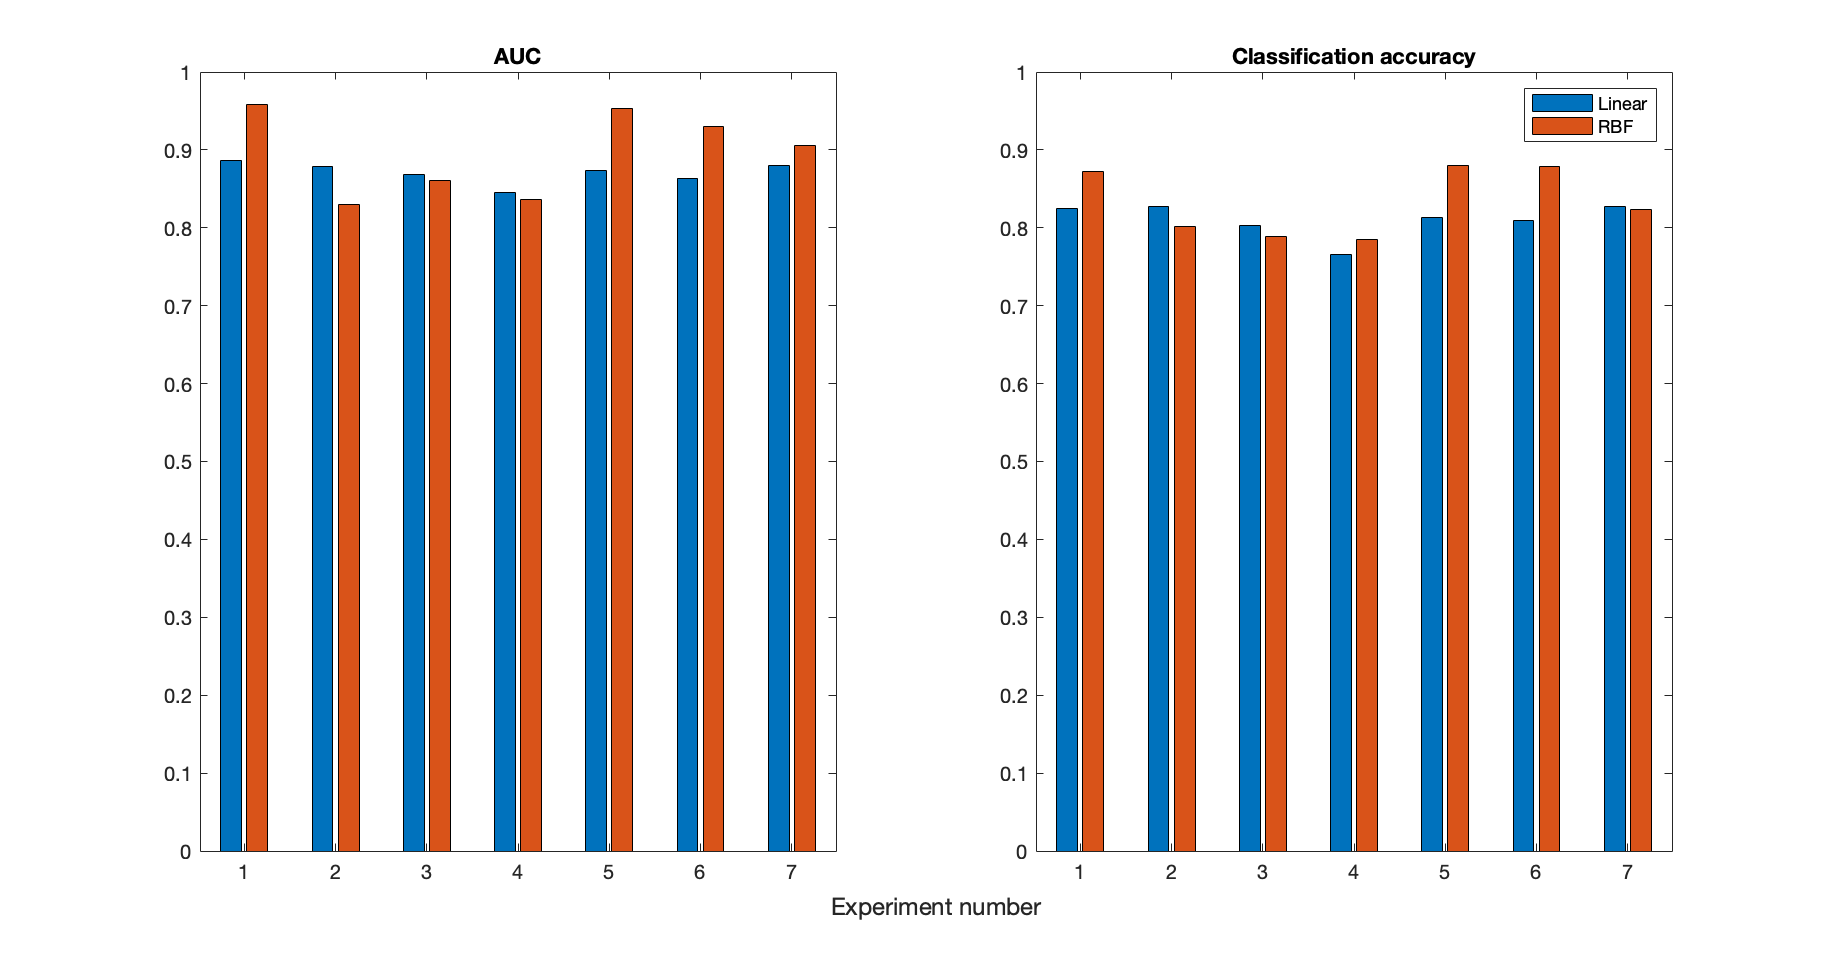
\includegraphics[width=\textwidth]{figures/hyp1_mfcc.png}
  \caption{The AUC and classification accuracy scores for linear and RBF models
  for different experiments for MFCC.}\label{fig:hyp1_mfcc}
\end{figure}

As shown in the table and chart, both evaluation metrics are around their
maximum in the control experiment (Experiment 1). Experiment 5 returns
comparable metrics to the control experiment, with slight improvements made to
the classification accuracy for the RBF model, but a slight reduction in the
AUC\@. The RBF model shows a clear reduction in performance for wider frequency
ranges across both evaluation metrics.

\subsection{GTCC}

The key parameter under test in this work as mentioned in
Section~\ref{sssec:gtcc} is the \textit{FrequencyRange} argument. 4 experiments were
devised and evaluated in order to see if any improvements to binary bird
classification models utilising GTCC could be made with adjusted
\textit{FrequencyRange} arguments. The experiments are listed in
Table~\ref{table:h1_gtcc_experiments}.

\begin{table}[h!t]
\begin{center}
\begin{tabular}{c c}
\toprule
Number & Frequency range (Hz) \\ [0.5ex]
\midrule
1 & 50 --- $\text{fs}/2$ \\
2 & 100 --- 7000 \\
3 & 50 --- 10000 \\
4 & 400 --- 6000 \\
\bottomrule
\end{tabular}
\caption{Description of experiments used for testing H1 with
GTCC.}\label{table:h1_gtcc_experiments}
\end{center}
\end{table}

\subsubsection{Comments on experiment setup}

As with the MFCC experiment, `fs' refers to the frequency sampling rate for a
given audio file. $\text{fs}/2$ is the maximum possible value for the
\textit{FrequencyRange} argument. By default the filter bank is a gammatone
filter bank, which can be visualized in figure. Note that it's not possible to
change the number of bands used by \texttt{gtcc}.

<figure of gammatone filterbank>

The experiment design was motivated as follows:

\begin{itemize}

  \item [Exp 1:] These are the defaults provided with the \texttt{gtcc} function
    and acts as a control experiment.

  \item [Exp 2:] This more closely matches the effective frequency range for the
    control experiment for \texttt{mfcc}, which obtained the best evaluation
    metrics. This range matches human speech and contains most birdsong
    frequencies.

  \item [Exp 3:] Similar to Experiment 2, but widens the range to account for
    frequencies outside of Experiment 2's range.

  \item [Exp 4:] Similar to Experiment 2, but tightens the range to achieve more
    discriminatory power.

\end{itemize}

\subsubsection{Results}

The results for the AUC and classification accuracy for GTCC can be seen in
Table~\ref{table:hyp1_gtcc} and can be visualized in Figure~\ref{fig:hyp1_gtcc}.

\begin{table}[h!t]
\begin{center}
\begin{tabular}{cc c|c c}
\toprule
& \multicolumn{2}{c|}{AUC} & \multicolumn{2}{c}{Accuracy} \\
  Experiment & Linear & RBF & Linear & RBF \\ [0.5ex]
\midrule
  1 & 0.884 & 0.895 & 0.844 & 0.802 \\
  2 & 0.887 & 0.946 & 0.831 & 0.856 \\
  3 & \cellcolor{lightgray} 0.891 & 0.933 & \cellcolor{lightgray} 0.852 & 0.850 \\
  4 & 0.883 & \cellcolor{lightgray} 0.948 & 0.846 & \cellcolor{lightgray} 0.859 \\
\bottomrule
\end{tabular}
\caption{The AUC and classification accuracy scores for linear and RBF models
for different experiments for GTCC\@. The highest evaluation scores for each metric
and for each model are highlighted in grey.}\label{table:hyp1_gtcc}
\end{center}
\end{table}

\begin{figure}[ht]
  \centering
  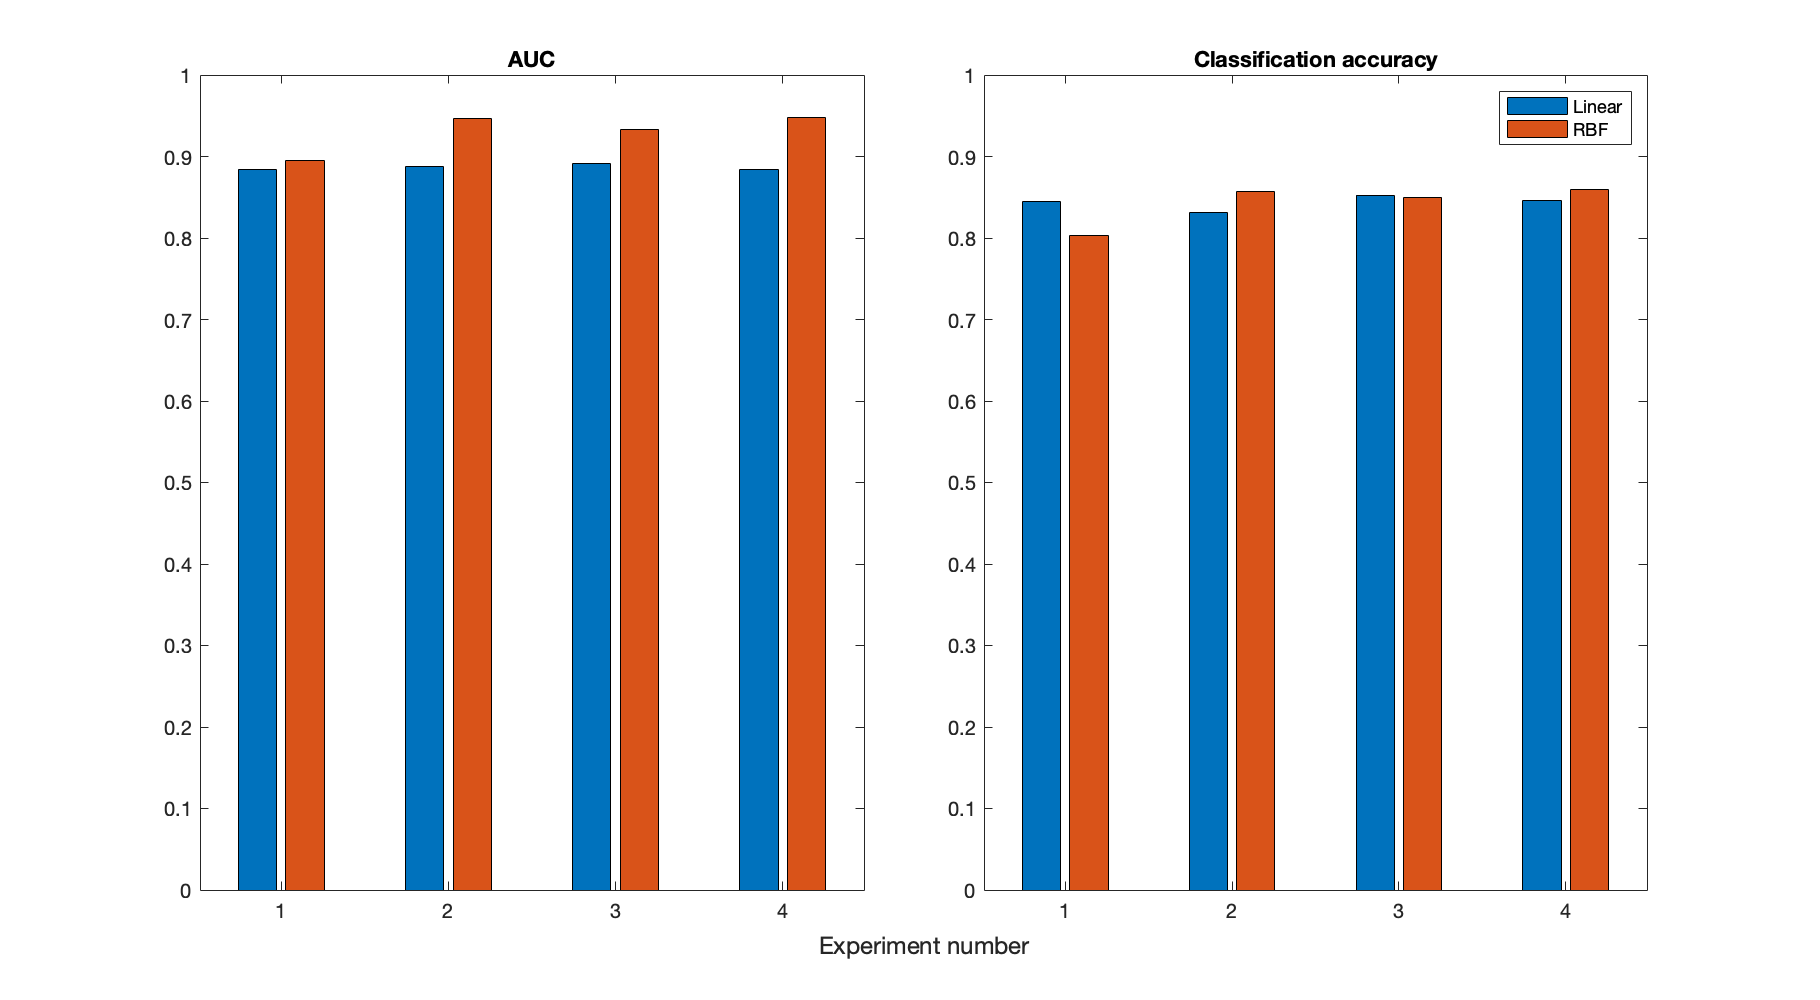
\includegraphics[width=\textwidth]{figures/hyp1_gtcc.png}
  \caption{The AUC and classification accuracy scores for linear and RBF models
  for different experiments for GTCC.}\label{fig:hyp1_gtcc}
\end{figure}

As shown in the table and chart, there is a significant increase in both metrics
for the RBF model when the frequency range is narrowed to be closer to the human
and birdsong vocalization range. The evaluation metrics for the linear model
remains largely similar across different frequency ranges.

\section{Hypothesis 2}

Hypothesis 2 (H2) is stated as follows:

\begin{quote}
Explore the performance of deep learning architectures such as Recurrent Neural
Networks (RNN) and Convolutional Neural Networks (CNN) and compare the results
with simpler statistical models. The hypothesis is that more complex and
flexible architectures such as these will have superior performance when
compared to simpler statistical models, such as SVMs.
\end{quote}

\subsection{CNN}

From the literature review described in Section~\ref{sssec:method:cnn}, we
propose the CNN architectures listed in Table~\ref{table:cnn_architectures} to
be tested and their performance evaluated against the baseline: the highest
performing models from H1.

\begin{table}[h!t]
\begin{center}
\begin{tabular}{l l l}
\toprule
Model 0 & Model 1~\cite{ruff2020automated} & Model 2~\cite{kahl2017large} \\[0.5ex]
2 weighted layers & 6 weighted layers & 8 weighted layers \\[0.5ex]
ReLU activation & ReLU activation & ELU activation \\[0.5ex]
Glorot initialization & Glorot initialization & He initialization \\[0.5ex]
$\sim$3s per epoch & $\sim$60s per epoch & $\sim$165s per epoch \\[0.5ex]
\midrule
\textbf{Conv1, $20 \times 5 \times 5$} &
\textbf{Conv1, $32 \times 3 \times 3$} &
\textbf{Conv1, $32 \times 7 \times 7$, Stride 2} \\
& MaxPooling, Size 2 & MaxPooling, Size 2 \\
& Dropout, $p=0.2$ & \\[1ex]
\textbf{DenseLayer, 2 Units} &
\textbf{Conv2, $32 \times 3 \times 3$} &
\textbf{Conv2, $128 \times 5 \times 5$, Stride 1} \\
Softmax Output & MaxPooling, Size 2 & MaxPooling, Size 2 \\
& Dropout, $p=0.2$ & \\[1ex]
& \textbf{Conv3, $64 \times 3 \times 3$} &
\textbf{Conv3, $256 \times 3 \times 3$, Stride 1} \\
& MaxPooling, Size 2 & MaxPooling, Size 2 \\
& Dropout, $p=0.2$ & \\[1ex]
& \textbf{Conv4, $64 \times 3 \times 3$} &
\textbf{Conv4, $512 \times 3 \times 3$, Stride 1} \\
& MaxPooling, Size 2 & MaxPooling, Size 2 \\
& Dropout, $p=0.2$ & \\[1ex]
& \textbf{DenseLayer, 64 Units} &
\textbf{Conv4, $512 \times 3 \times 3$, Stride 1} \\
& Dropout, $p=0.5$ & MaxPooling, Size 2 \\[1ex]
& \textbf{DenseLayer, 2 Units} &
\textbf{DenseLayer, 512 Units} \\
& Softmax output & Dropout, $p=0.5$ \\[1ex]
& & \textbf{DenseLayer, 512 Units} \\
& & Dropout, $p=0.5$ \\[1ex]
& & \textbf{DenseLayer, 2 Units} \\
& & Softmax output \\[1ex]
\bottomrule
\end{tabular}
\caption{Candidate CNN architectures.}\label{table:cnn_architectures}
\end{center}
\end{table}
